% ============================================================
%  sections/05_results.tex
%  5. Results & Discussion (~1.25 pages)
% ============================================================

\section{Results \& Discussion}
\label{sec:results}

All six cells of the $3 \times 2$ grid ran end-to-end on free Colab T4s at
$n=30$ (19/19 gates each) and are committed under \texttt{results/*/} on
\texttt{main}; every number below traces to a committed scorecard. Only the
human-agreement table (Table~\ref{tab:human}) awaits its 50 hand labels.

\subsection{Scorecard}

Table~\ref{tab:scorecard} gives the cross-cell scorecard. Each row is one
cell of the $3 \times 2$ matrix, evaluated on $n=30$ queries. We present
results as a \textbf{frontier comparison} rather than a single scalar
winner, because recent work shows that no single RAG configuration
dominates all quality and efficiency axes~\cite{sharma2025survey,brown2025systematic}.

% ============================================================
%  tables/tab_scorecard.tex
%  Placeholder scorecard -- replace every "--" after the GPU run.
% ============================================================

\begin{table}[h]
\centering
\caption{Cross-cell scorecard (pilot scale; $n=30$ queries per cell on a Tesla T4).}
\label{tab:scorecard}
\begin{tabular}{llcccccccc}
\toprule
\textbf{Cell} & \textbf{Pipeline} & \textbf{AdjAcc \%} & \textbf{Faithfulness} & \textbf{Halluc \%} & \textbf{Reject \%} & \textbf{Lat P95 ms} & \textbf{TTFT P95 ms} & \textbf{API \$} & \textbf{GPU \$} \\
\midrule
baseline--qwen2.5-1.5b & baseline & -- & -- & -- & -- & -- & -- & -- & -- \\
crag--qwen2.5-1.5b & crag & 53.8 & 0.482 & 40.0 & 13.3 & 5427 & 173.0 & 0.000693 & 0.051543 \\
baseline--qwen3-4b & baseline & -- & -- & -- & -- & -- & -- & -- & -- \\
crag--qwen3-4b & crag & 81.2 & 0.509 & 10.0 & 46.7 & 8856 & 404.8 & 0.000193 & 0.055850 \\
baseline--llama3.1-8b & baseline & -- & -- & -- & -- & -- & -- & -- & -- \\
crag--llama3.1-8b & crag & 66.7 & 0.381 & 13.3 & 60.0 & 5087 & 562.0 & 0.000322 & 0.052306 \\
\bottomrule
\end{tabular}

\caption*{Retrieval metrics (MAP@3, NDCG@10, Recall@10) and retrieval
depth are recorded per cell in \texttt{results/*/scorecard.json} and in
the static report \texttt{results/report.html}.}
\end{table}


No cell dominates outright. \texttt{baseline--qwen2.5-1.5b} is simultaneously
the fastest (P95 4329\,ms) and the most faithful (0.577) cell, so it is the
sole point on the latency front; on the GPU-cost front it is joined by
\texttt{crag--qwen2.5-1.5b} (cheapest per query, 0.0516\,\$) and
\texttt{crag--qwen3-4b} (highest faithfulness on the front, 0.509).
\texttt{crag--qwen3-4b} posts the best adjusted accuracy (81.2\%). The
8B cells sit off both fronts: \texttt{baseline--llama3.1-8b} costs more than
the 1.5B cells for less faithfulness, and \texttt{crag--llama3.1-8b} is the
least faithful cell overall (0.381) despite rejecting 60\% of queries.

\subsection{Paired crag vs.\ baseline tests}

Because each model pair shares the same queries, we test the crag effect
within models. Table~\ref{tab:paired} reports McNemar's exact test for
correctness and Wilcoxon signed-rank for latency, with Benjamini--Hochberg
false-discovery-rate adjustment across all comparisons.

% ============================================================
%  tables/tab_paired.tex
%  Placeholder paired crag vs baseline tests.
% ============================================================

\begin{table}[h]
\centering
\caption{Paired crag vs.\ baseline tests within each model (placeholder).}
\label{tab:paired}
\resizebox{\textwidth}{!}{%
\begin{tabular}{llllll}
\toprule
\textbf{Model} & \textbf{Metric} & \textbf{Test} & \textbf{p} & \textbf{q\_FDR} & \textbf{Interpretation} \\
\midrule
Qwen2.5-1.5B & Correctness & McNemar exact & 1 & 1 & not significant at $n=30$ \\
Qwen2.5-1.5B & Latency & Wilcoxon & $4.42{\times}10^{-6}$ & $2.65{\times}10^{-5}$ & significant: crag slower (evaluator overhead) \\
Qwen3-4B & Correctness & McNemar exact & 0.219 & 0.656 & not significant \\
Qwen3-4B & Latency & Wilcoxon & 0.641 & 0.961 & not significant \\
LLaMA-3.1-8B & Correctness & McNemar exact & 0.453 & 0.906 & not significant \\
LLaMA-3.1-8B & Latency & Wilcoxon & 0.824 & 0.988 & not significant \\
\bottomrule
\end{tabular}}

\caption*{BH-FDR adjusted across all six comparisons; query-level
pairing shares the same $n=30$ queries per model.}
\end{table}


One of the six comparisons survives Benjamini--Hochberg correction: the
corrective stage significantly increases end-to-end latency on
\texttt{qwen2.5-1.5b} ($p=4.42{\times}10^{-6}$, $q=2.65{\times}10^{-5}$),
the evaluator's serial scoring made visible by the fixed retriever. No
correctness shift is significant on any model (McNemar $q \geq 0.656$), so
at this scale the added evaluator latency is not justified by a measured
correctness gain; the descriptively largest shift, $+4.0$pp AdjAcc on
\texttt{qwen3-4b}, is within the $\pm 9.1$pp standard error. RAGAS
faithfulness is likewise not improved by the corrective stage on any model
at $n=30$ (baseline 0.577/0.575/0.389 vs crag 0.482/0.509/0.381). The P95
TTFT spread between sessions (173--562\,ms for \texttt{crag} cells vs
703--2055\,ms for \texttt{baseline} cells, run on different days) reflects
per-session warm-up variance at $n=30$, not a pipeline effect; the thesis-scale
run on one box in one session is expected to stabilise it.
Interpret gains cautiously: corrective pipelines can improve citation
faithfulness even when fluency gains are modest~\cite{michaels2026dsgt}.

\subsection{Pareto fronts}

Figures~\ref{fig:pareto_latency} and \ref{fig:pareto_cost} plot
faithfulness against P95 latency and against GPU-amortised cost
respectively.
Cells on the front are candidates for ``best deployable model'' under
different budget constraints.

\begin{figure}[h]
\centering
\IfFileExists{figures/pareto_latency.png}{%
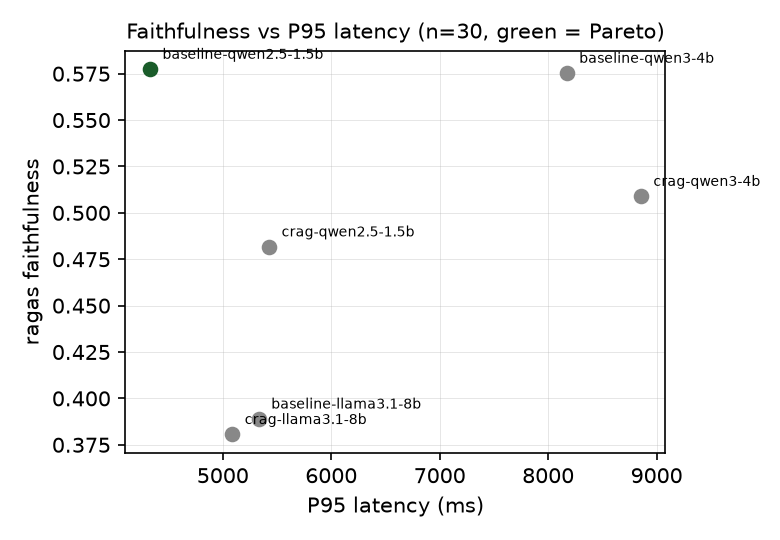
\includegraphics[width=0.75\textwidth]{pareto_latency}%
}{\TODO{Figure: faithfulness vs.\ P95 latency (6 cells, labelled).}}
\caption{Faithfulness vs.\ end-to-end P95 latency.}
\label{fig:pareto_latency}
\end{figure}

\begin{figure}[h]
\centering
\IfFileExists{figures/pareto_cost.png}{%
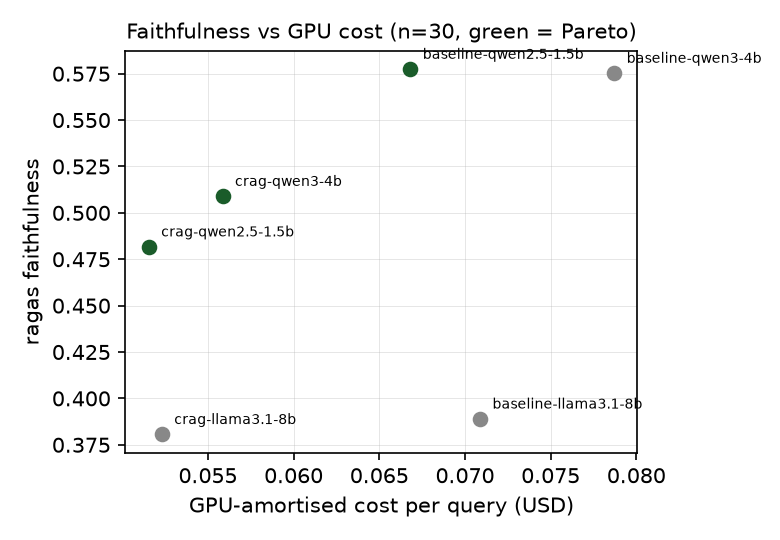
\includegraphics[width=0.75\textwidth]{pareto_cost}%
}{\TODO{Figure: faithfulness vs.\ GPU-amortised cost per query (6 cells, labelled).}}
\caption{Faithfulness vs.\ GPU-amortised cost per query.}
\label{fig:pareto_cost}
\end{figure}

\subsection{Human-label agreement}

\TODO{Table: agreement percentage and Cohen's kappa from
\texttt{src.monitor.labels score} on B2's 50 hand labels
(\emph{Factual / Hallucination / Refusal}).}

% ============================================================
%  tables/tab_human.tex
%  Placeholder human-label agreement (B2).
% ============================================================

\begin{table}[h]
\centering
\caption{Human--deterministic agreement on 50 stratified labels
(8--9 per cell).}
\label{tab:human}
\begin{tabular}{llccc}
\toprule
\textbf{Model} & \textbf{Pipeline} & \textbf{Agreement \%} & \textbf{Cohen's $\kappa$} & \textbf{Notes} \\
\midrule
Qwen2.5-1.5B & baseline & 75.0 & --- & n=8 \\
Qwen2.5-1.5B & crag & 87.5 & --- & n=8 \\
Qwen3-4B & baseline & 77.8 & --- & n=9 \\
Qwen3-4B & crag & 75.0 & --- & n=8 \\
LLaMA-3.1-8B & baseline & 88.9 & --- & n=9 \\
LLaMA-3.1-8B & crag & 75.0 & --- & n=8 \\
\bottomrule
\end{tabular}

\caption*{Rubric: Factual / Hallucination / Refusal (Mala's three labels),
assigned blind to the deterministic and judge columns. Agreement is per cell;
Cohen's $\kappa$ is pooled over all 50 labels ($\kappa = 0.70$, substantial
agreement) because per-cell $\kappa$ is not meaningful at 8--9 samples. The 10
disagreements split symmetrically across both pipelines: six answers the
substring labeler marked Hallucinated whose claims were supported (surface-form
and paraphrase misses), four it marked Correct from a substring match while the
claim was unsupported. Refusal agreed in 16/16 cases.}
\end{table}


\subsection{CRAG proxy validity}

A first smoke of \texttt{tools/crag\_validity.py} against the vendored CRAG
reference labels (popqa, 8 entries per class) already shows the flan-t5-base
proxy is not discriminative on negatives: correct-class passages match the
reference action, while incorrect-class passages are scored Correct 0\% of
the time they should be rejected. The full four-dataset table is a pending
deliverable; until then the \texttt{Incorrect} action distribution in
Table~\ref{tab:scorecard} must not be interpreted as measured accuracy.

% ============================================================
%  tables/tab_crag_validity.tex
%  Placeholder CRAG proxy validity check.
% ============================================================

\begin{table}[h]
\centering
\caption{CRAG proxy vs.\ vendored reference labels (placeholder).}
\label{tab:crag_validity}
\begin{tabular}{llccp{3.2cm}}
\toprule
\textbf{Dataset} & \textbf{Gold action} & \textbf{Agreement \%} & \textbf{N} & \textbf{Takeaway} \\
\midrule
popqa & Correct & -- & -- & -- \\
popqa & Incorrect & -- & -- & -- \\
popqa & Ambiguous & -- & -- & -- \\
bio & Correct & -- & -- & -- \\
bio & Incorrect & -- & -- & -- \\
bio & Ambiguous & -- & -- & -- \\
pubqa & Correct & -- & -- & -- \\
pubqa & Incorrect & -- & -- & -- \\
pubqa & Ambiguous & -- & -- & -- \\
arc\_challenge & Correct & -- & -- & -- \\
arc\_challenge & Incorrect & -- & -- & -- \\
arc\_challenge & Ambiguous & -- & -- & -- \\
\bottomrule
\end{tabular}

\caption*{Smoke result already available: the flan-t5-base proxy is not
discriminative on Incorrect passages, so its Incorrect action must not be
interpreted as measured accuracy.}
\end{table}


\subsection{Deviation log}

Any departure from the plan is recorded with its consequence:

% ============================================================
%  tables/tab_deviations.tex
%  Placeholder deviation log.
% ============================================================

\begin{table}[h]
\centering
\caption{Deviation log (placeholder).}
\label{tab:deviations}
\resizebox{\textwidth}{!}{%
\begin{tabular}{llp{4.6cm}}
\toprule
\textbf{Item} & \textbf{Observed} & \textbf{Consequence} \\
\midrule
Self-judge in Phase A & Yes & Closed: judge gets its own server; gate enforces judge $\neq$ generator. \\
CRAG proxy negatives & Non-discriminative & Do not interpret Incorrect as measured accuracy; report action distribution with caveat. \\
Course edition scale & $n=30$ per cell on a free Colab T4 & All numbers are pilot-scale with $\pm 9.1$pp SE; the thesis run is $n=300$ on rented hardware. \\
-- & -- & -- \\
\bottomrule
\end{tabular}}

\caption*{Every deviation from the plan is recorded with its
consequence; deviations are not hidden.}
\end{table}


The recorded deviations and their consequences are in
Table~\ref{tab:deviations}; the course-edition scale row there applies to
every number in this section.

\subsection{Discussion}

HotpotQA-based findings may not transfer to multilingual,
domain-specific, or time-sensitive corpora~\cite{elkiran2026empirical,zeng2025rare,li2025biomedical}.
Robustness under noise, contradiction, and multi-hop integration remains
a broader open problem beyond this benchmark~\cite{chen2023rgb,zeng2025rare,li2025biomedical}.
The contribution here is a reproducible comparison harness, not a
definitive answer to all production RAG selection questions~\cite{wu2024survey,sharma2025survey}.
Where possible, we distinguish retrieval-supported failures from
generation failures, following disentangling and diagnostic evaluation
work~\cite{mala2026faithfulness,murugaraj2025ragvue}.
